\section{Arquitectura del sistema}\label{section:arquitecturaSistema}
A grandes rasgos, existe en el medio del sistema una aplicación en la nube denominada \emph{Nube de Conductores} que se encarga de hacer llegar los mensajes procedentes de los ciclistas a los vehículos a motor, y los mensajes enviados por los vehículos a motor a los ciclistas. Además, filtra los mensajes que han sido mal formados, monitoriza las posiciones de todos los vehículos en la carretera y es capáz de predecir cuándo se puede dar la posibilidad de que haya un choque entre dos vehículos; en cuyo caso avisa a los conductores de esta posibilidad.

Los vehículos a motor mandan continuamente beacons a través de un \gls{obu} anunciando su posición, velocidad y la dirección a la que se dirigen. No se comunican directamente con la \emph{Nube de Conductores}, sino que los mensajes enviados son escuchados por una unidad desplegada en carretera llamada \gls{rsu}. Esta última recoge los mensajes que escucha y los reenvía a la nube por conectividad 3G.

Por otro lado, los ciclistas envían información a la \emph{Nube de Conductores} a través de 3G o 4G; dependiendo de la disponibilidad. Éstos también pueden agruparse empleando \emph{Wi-Fi 802.11}, mediante la creación de un \emph{HUB} de dispositivos móviles en el cual se envían notificaciones sobre los eventos que aparezcan.

En la figura \ref{fig:ArquitecturaSistema} se puede observar de qué elementos está compuesto el sistema y cómo se comunican entre ellos. Como puede apreciarse, hay diferentes tecnologías de comunicación y desarrollo en cada una de las plataformas, por lo que uno de los requisitos es que la solución desarrollada sea flexible a los cambios de tecnología.

\begin{figure}[H]
	\begin{center}
		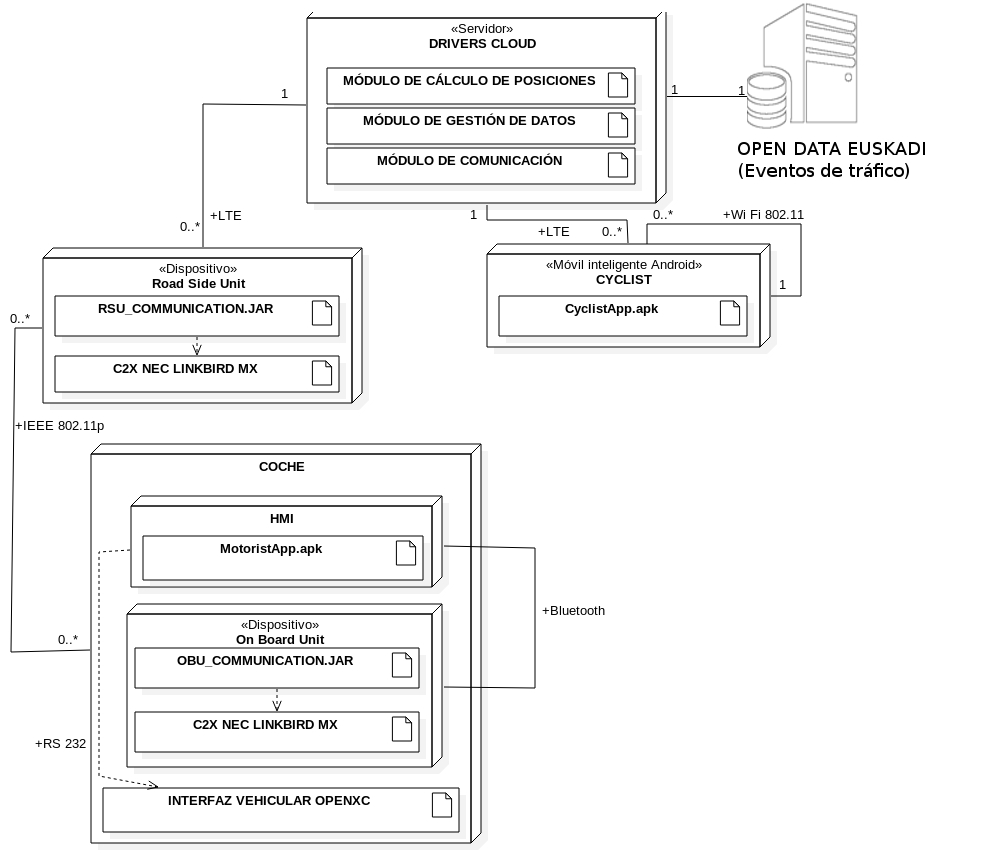
\includegraphics[scale=0.4]{arquitectura_global}
		\caption{Arquitectura del sistema}
		\label{fig:ArquitecturaSistema}
	 \end{center}
\end{figure}
